\documentclass[11pt, oneside]{article}   	% use "amsart" instead of "article" for AMSLaTeX format
\usepackage[margin=1in]{geometry}                		% See geometry.pdf to learn the layout options. There are lots.
\geometry{letterpaper}                   		% ... or a4paper or a5paper or ... 
%\geometry{landscape}                		% Activate for for rotated page geometry
\usepackage[parfill]{parskip}    		% Activate to begin paragraphs with an empty line rather than an indent
\usepackage{graphicx}				% Use pdf, png, jpg, or eps� with pdflatex; use eps in DVI mode
\usepackage{lipsum}
\usepackage{hyperref}
\usepackage{cleveref}				% TeX will automatically convert eps --> pdf in pdflatex		
\usepackage{amssymb}
\usepackage{sectsty}


\sectionfont{\fontsize{12}{15}\selectfont}

\newcommand{\la}{\emph{Later }}
\newcommand{\now}{\emph{Now }}


\title{Parallel Path Finding Literature Survey}
\author{Stephan Boettcher}
%\date{}							% Activate to display a given date or no date

\begin{document}

\maketitle
\begin{figure} [!h]
  \centering
    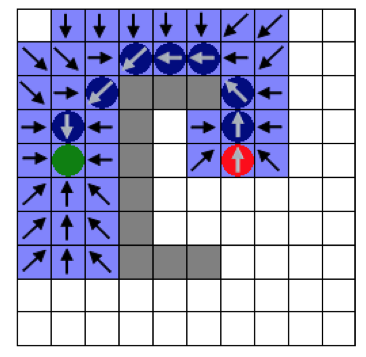
\includegraphics[width=0.5\textwidth]{moo.png}
\end{figure}
\newpage
\section*{Introduction}
Path finding algorithms were created early in  field of computer science, first with Dijkstra's algorithm (1959), and later with the creation of the A* algorithm (1968). The A* algorithm uses  a distance-plus-cost heuristic function to determine the order which graph nodes are visited while searching for the optimal path, if it exists, from point A to point B. To do this, the A* algorithm traverses a graph, following a path of lowest know heuristic cost while keeping a sorted list of alternative path segments\cite{Dong}. The result is the least-cost path from the initial node to the target node is chosen out of the sorted list as the shortest path, thereby guaranteeing an optimal path between the nodes. This method of path-finding has popular in gaming, logistics, navigation, CAD systems\cite{Szabo}, and mission planning since its creation. As hardware systems continue to improve, the use of A* path finding algorithms in games, such as Massive Multi-Player On-line Role Playing Games (MMORPG), has increased\cite{Botea}\cite{Inam}\cite{Gedge}\cite{Nohra}\cite{McNally}\cite{Szabo}. However, as the number of Artificial Intelligence (AI) players increase, the computational load of creating and maintaining paths for these characters over complex terrain has increased drastically. In its current state, the A* algorithm does not scale well to multiple processors of a distributed architecture\cite{Accaputo}. Many gaming platforms currently dedicated threads and processor cores to just calculate A* paths\cite{Nohra} as a lazy method of 'parallelizing'. Attempts have been made to directly parallelized the A* algorithm \cite{Accaputo} but ended poorly. Other researchers have focused on other path finding algorithms based on A*\cite{Brand}.

\section*{Parallelization of the A* Algorithm}
The goal of parallelizing the A* algorithm is to achieve the greatest amount of speedup to minimize the algorithm runtime. A number of different modifications to the Dijkstra algorithm (of which, A* is a subset) to achieve this speedup. Because the A* algorithm needs to maintain a sorted open list, and thus may need to correct said list as nodes are opened and closed, achieving a good scale up of the algorithm is difficult. By using the Hierarchical A* Algorithm and using OpenMP, speedups can be achieved but are challenging due load balancing issues\cite{Miller}. An easy way to involve two cores in the A* search is to begin the search at both end nodes in a Parallel Bidirectional Search(PBS)\cite{Brand}. While the PBS algorithm employs the same A* algorithm, as the serial version, it is possible that the path in the area around the intersection is not strictly optimal, as not all nodes around the intersection may be fully flooded.

Another method seen in the literature to achieve speedups is the use of pre-stored paths. If the A* algorithm has been run on an area, so long as no changes have occurred on the path length (e.g. dynamic barriers), there is no need to recompute the length. Another implementation of the A* uses 'multiple threads per agent\cite{Inam} to work on a small subset of the path as a group. A master thread maintains control of the execution and executes the choice of 'current node'. Thread synchronization is required for this version, resulting in a number of threads sitting idle while the master thread executes the serial code. Another way to achieve speedups of the A* algorithm is to 'find the A* oath hierarchically\cite{Botea}.  This 'multiple thread per agent' algorithm must have an modified termination condition from that of the A* method. The program must not terminate immediately upon finding a path or else it may report a suboptimal solution, instead it is suggested that a global flag should be set to true indicating that  a path has been found\cite{Cohen}.

\section*{Other Parallel Path Finding Algorithms}  
A path finding algorithm's goal is to find the optimal path from point A to point B. However, if the constraint of strict optimality can be relaxed, large gains in performance can be realized. All of the following algorithms described are based off of the A* search or are in the same family as the A* search. 

A Fringe Search (FS) is based off of an A* algorithm, but instead of maintaining a sorted list of open and closed nodes, it uses a \now list and a \la list. The \now and \la lists do not need to be sorted and thus cut out a costly portion of the A* algorithm. Because the nodes are not sorted, nor does the FS need to maintain any kind of sorted array, the path that is ultimately generated is no longer guaranteed to be optimal\cite{Brand}. However, studies have shown that the FS algorithm is usually within a few percentage points of being optimal. The FS algorithm also lends itself to being scaled up and parallelized more readily than the A* algorithm. The first way is with the Distributed Fringe Search (DFS). The DFS takes the \now nodes in the FS algorithm and disburses them over multiple cores. Each core then computes the smallest f(n) value found locally and pass that value to a master core to do comparisons. A drawback of the DFS algorithm is that the it is no longer possible to keep track of the parent-child relation of nodes during flooding. This information is needed to reconstruct the resulting path. As a result, a shared buffer must be used to signal to each other who is the owner. Care must be taken to avoid race conditions in the shared buffer, which may cause a drop in performance\cite{Brand}. 

Another way to utilize the cores available in a CPU or GPU is to have each core find a small segment of the overall path. This can be done if a high-level graph is first generated to create potential waypoints on the route. Once the high-level graph has been created, a Parallel Hierarchic Search (PHS) can then be implemented. A PHS creates a path through the high-level graph and then find sub paths connecting the anchor nodes. A "beautification" step is then applied to create way-points half way between the path segment nodes to help find "shortcuts" between the high-level anchor  waypoint nodes. The path segments are then calculated over multiple cores. The PHS suffers from a 'critical section' in the code that is required to allow safe access to selecting path segments and returning path segment solutions. This can greatly impact the performance of the algorithm. The Parallel Ripple Search (PRS) attempts to remedy this. The PRS uses the same high-level graph as the PHS but now finds path segments doing a normal A*-like search to the nearest neighbors. As each core foods the graph, the 'ripples' will eventually overlap and hopefully shortcuts can be uncovered. The PRS is also good at dealing with dynamic obstacles in the path\cite{Brand}. 

\section*{Conclusion}
There are a number of ways and methods in the literature for how to attack the problem of parallelizing the A* algorithm. Some focus on maintaining strict optimality while others relax this constraint to realize gains in computational performance. For the application of a drone attempting to travel from point A to point B, small deviations and a semi-suboptimal path would be acceptable, so long as the path didn't vary too far from optimal. 








\pagebreak
\begin{thebibliography}{99} 
\addcontentsline{toc}{section}{References} 

\bibitem{Accaputo}  Accaputo, Giuseppe, and Pascal Iselin. "Parallel A* Pathfinding Algorithm." SPCL - Scalable Parallel Computing Lab. ETH Z�rich, 16 Dec. 2013. Web. 1 Oct. 2014. 

\bibitem{Allen} Allen, T. L. (2011). Time-optimal active decision making. Thesis. Retrieved 1 Oct. 2014. 

\bibitem{Brand} Brand, S., \& Bidarra, R. (2012). Multi-core scalable and efficient pathfinding with parallel ripple search. Computer Animation and Virtual Worlds, 23(2), 73-85. doi:10.1002/cav.1427 13 Oct. 2014. 

\bibitem{Botea} Botea, A., M�ller, M., \& Schaeffer, J. (2004). Near optimal hierarchical path-finding. Journal of Game Development, 1(1), 7-28. Retrieved 13 Oct 2014

\bibitem{Cohen} Cohen, D., \& Dallas, M. (2010). Implementation of parallel path finding in a shared memory architecture. Department of Computer Science Rensselaer Polytechnic Institute: Troy, NY. Retrieved 1 Oct. 2014. 

\bibitem{Dong} Dong, G., Fu, X., \& Xue, H. (n.d.). An improved A* algorithm and implementation for pathfinding in symmetrical circumstances. Retrieved 1 Oct. 2014. 

\bibitem {Gedge} Gedge, J. (n.d.). Parallel search for map-based pathfinding. Retrieved 1 Oct. 2014. 

\bibitem{Inam} Inam, R. (2010). A* algorithm for multi-core graphics processors. Thesis. Retrieved 1 Oct. 2014. 

\bibitem {McNally} McNally, O. (2010). Multi-Agent pathfinding over real-world data using CUDA. Retrieved 1 Oct. 2014. 

\bibitem{Miller} Miller, W. (n.d.). Applying parallel programming to path-finding with the A* algorithm. Applying parallel programming to path-finding with the A* algorithm 1 Oct. 2014. 

\bibitem{Nohra} Nohra, J., \& Champandard, A. J. (2010). The secrets of parallel pathfinding on modern computer hardware. Intel Software Network, Intel Corp. Retrieved 1 Oct. 2014. 

\bibitem{Phipps} Phipps, A. K. (2004). Parallel algorithms for geometric shortest path problems. Master of Science Computer Science School of Informatics University of Edinburgh. Retrieved 1 Oct. 2014. 

\bibitem {Szabo} Szab\'o, C., \& Sobota, B. (n.d.). Path-Finding algorithm application for route-searching in different areas of computer graphics. Retrieved 1 Oct. 2014. 

\bibitem{ Standley} Standley, T., \& Korf, R. (2011). Complete algorithms for cooperative pathfinding problems. In IJCAI (pp. 668-673). Retrieved 1 Oct. 2014. 





 \end{thebibliography}


%%% End document
\end{document}